\chapter{Continuous Delivery}
\label{chap:continuousDelivery}
Martin Fowler schreibt \cite{Fowler:CD}:
\\
"`Continuous Delivery is a software development discipline where you build software in such a way that the software can be released to production at any time. [..] You achieve continuous delivery by continuously integrating the software done by the development team, building executables, and running automated tests on those executables to detect problems. Furthermore you push the executables into increasingly production-like environments to ensure the software will work in production. To do this you use a Deployment Pipeline."' 
\\
Wie von Martin Fowler zu lesen ist, ist Continuous Integration ein Teilprozess von Continuous Delivery und beschreibt dessen Grundlagen. Bevor Continuous Delivery genauer erläutert werden kann, muss zunächst der Begriff Continuous Integration erläutert werden.

\section{Continuous Integration}\
\label{subsec:ContinuousIntegration}
"`At all times you know where you are, what works, what doesn't, the outstanding bugs you have in your system "'\cite{Fowler:CI}. 
\\
Das ist die Aufgabe von Continuous Integration. Um dies zu erreichen ist es notwendig jede Teilaufgabe innerhalb der Entwicklung in den Prozess mit einzubinden. Das Ziel ist es so früh wie möglich Bugs zu erkennen und diese zu beheben. Dafür muss jeder Prozess automatisiert werden. Vor allem muss es möglich sein, Tests automatisiert durchführen zu können. Eine einfache Continuous Integration zeigt folgendes Bild:

\begin{figure}[htb]
    \centering 
    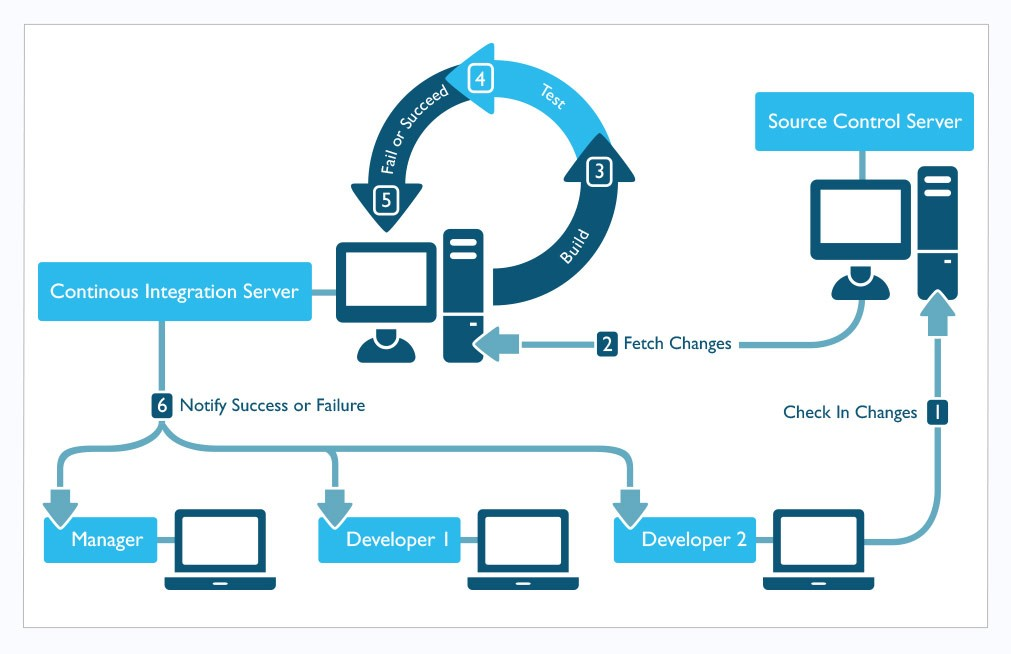
\includegraphics[width=\linewidth]{content/images/continuous_integration}\
    \quelle\url{https://insights.sei.cmu.edu/devops/2015/01/continuous-integration-in-devops-1.html}
    \caption[Continuous Integration]{Continuous Integration\\}
    \label{fig:ContinuousIntegration}  
\end{figure}\noindent 
Wie zu erkennen ist, sorgt ein zentraler "`Continuous Integration Server"' für das Bauen und Testen der Software und informiert die zuständigen Entwickler über den Status. In der Regel wird dies bei jeder Code Änderung durchgeführt, sodass direkt erkannt wird, ob eine Änderung des Codes zu einem Erfolg oder einem Fehlschlag führt.

Continuous Delivery ist eine natürliche Erweiterung von Continuous Integration. Trotzdem unterscheiden sich die beiden Begriffe nicht wirklich von einander. Während bei der Continuous Integration wert darauf gelegt wird, Software möglichst Fehlerfrei zu erzeugen, wird bei Continuous Delivery  darauf wert gelegt, Software möglichst regelmäßig zu deployen. Continuous Delivery beinhaltet Continuous Integration und erweitert diese um das ausliefern. In der nachfolgenden Sektion, wird noch einmal auf den unterschied zwischen Continuous Integration und Delivery eingegangen

\section{Continuous Delivery Pipeline}
\label{subsec:Continuous Delivery Pipeline}
Die Continuous Delivery Pipeline beschreibt die Teilprozesse, welche durchlaufen werden müssen, um Continuous Delivery durchführen zu können. Dabei wird die Pipeline automatisch durchlaufen. Die Folgende Abbildung zeigt eine mögliche Pipeline. Das Deployen in die Produktionsumgebungen "`PRODBLUE"' und "`PRODGREEN"' muss jedoch manuel, durch klicken auf Trigger, erfolgen.

\begin{figure}[htb]
    \centering 
    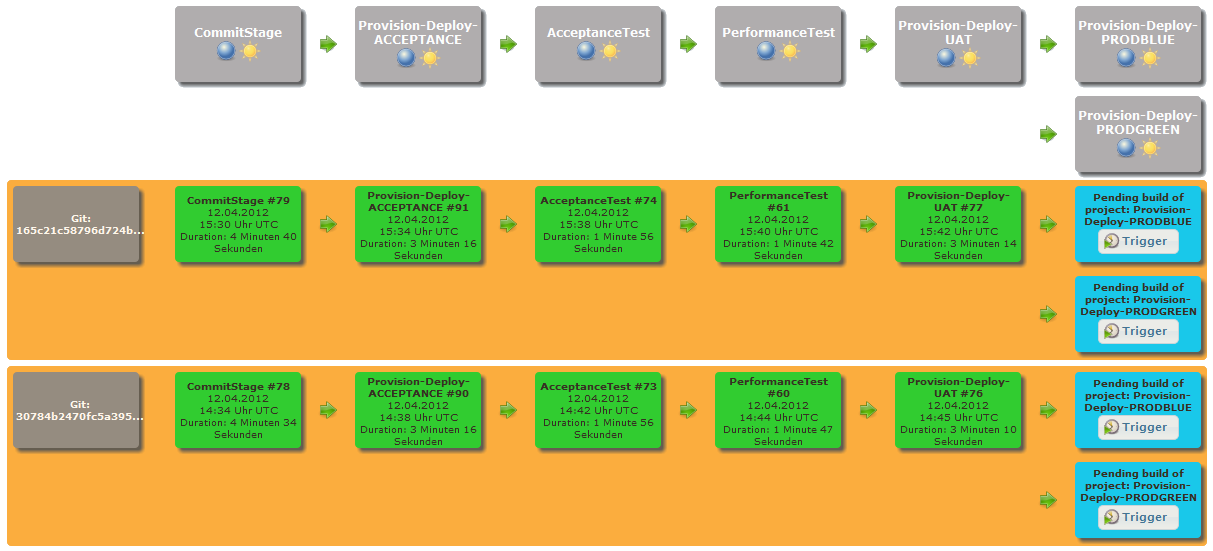
\includegraphics[width=\linewidth]{content/images/pipeline}\
    \quelle\url{https://blog.codecentric.de/en/2012/04/continuous-delivery-in-the-cloud-part1-overview/}
    \caption[Continuous Delivery Pipeline]{Continuous Delivery Pipeline\\}
    \label{fig:ContinuousDeliveryPipeline}  
\end{figure}\noindent 
Wie man in der Abbildung sehen kann beinhaltet die Pipeline alle nötigen schritte, welche zuvor in \nameref{subsec:ContinuousIntegration} besprochen wurden. Hier sei noch einmal erwähnt, dass Continuous Integration alle Prozesse, bis auf den letzten (das Deployment), beinhaltet. Continuous Integration und Delivery unterscheiden sich, wie schon zu vor erwähnt, nur beim letzten Schritt, dem Deployen. Dieser wird jedoch bei Continuous Delivery Manuel ausgeführt. Unter ausgeführt ist hierbei zu verstehen, dass ein Prozess, hier durch einen klick, gestartet wird, welcher die Software, bzw. das Artefakt, automatisch in die Produktion bringt.

\section{Einführung von Continuous Delivery}
\label{subsec:EinfuehrungCD}
In Kaptiel \ref{sec:problemstellung} \nameref{sec:problemstellung} wurde bereits ein Fall beschrieben, in der kein Continuous Delivery eingesetzt wird. Darauf aufbauend wird nun Schritt für Schritt die vorhandene Softwareentwicklung in Continuous Delivery überführt.
\\\\
Damit das Dependencie Management und automatisieren von Tests bzw. das ausführen zusätzlicher Aktionen erleichtert wird, wird zunächst ein Build-Management-Tool eingeführt. Dadurch wird sichergestellt, dass Software idempotent gebaut werden kann. Der Build-Prozess ist dadurch Standardisiert und kann beliebig oft wiederholt werden.
\\\\
Wie bereits erläutert wurde, ist in diesem Beispiel die Qualitätssicherung zwar ein Teil der Softwareentwicklung, jegliche Tests werden jedoch nur manuell ausgeführt, was zu regelmäßigen, unentdeckten Fehlern führt. Daher muss zunächst einmal dafür gesorgt werden, dass Unit-Tests geschrieben werden, welche vor dem Bauen der Software, die Code Qualität und Richtigkeit überprüft.  Test-Driven-Development (TDD)\footnote{TDD wird hier nur erwähnt und nicht weiter erläutert. Es sei auf Fachliteratur zu diesem Thema verwiesen.} ist einer der Möglichkeiten, sicherzustellen, dass Tests regelmäßig geschrieben werden. Zusammen mit dem eingeführten Build-Management-Tool können nun, vor dem Bauen der Software, die Unit Tests durchlaufen und dadurch der Code der Software überprüft werden.
\\\\
Nun ist zu mindestens Sichergestellt, dass diese Art der Tests automatisiert ablaufen und nicht mehr manuell durchgeführt werden müssen. Jedoch müssen noch Akzeptanz-, Performanz- und Integrations-Tests automatisiert werden. Diese Tests können jedoch nicht immer durch das Build-Management-Tool abgedeckt werden. Daher Wird nun ein "`Build and Management"' Werkzeug wie Jenkins\footnote{siehe: https://jenkins.io/} eingesetzt wird, welches sowohl die Software baut, unter anderem mit dem eingeführten Build-Management-Tool, als auch die anderen Tests abbilden kann. Wie die Software genau funktioniert, soll hier jedoch nicht weiter erläutert werden. Es sei nur erwähnt, dass es durch Konfiguration und Plugins möglich ist, die oben genannten Tests innerhalb von Jenkins abzubilden. Es wurde eine \textit{Continuous Delivery Pipeline} erschaffen. Die Abbildung \ref{fig:ContinuousDeliveryPipeline} \nameref{fig:ContinuousDeliveryPipeline} zeigt ein ausschnitt aus dem "`Build and Management"' Werkzeug Jenkins. Außerdem ist es durch Jenkins möglich jeden Schritt zu Überwachen und zu Protokollieren, sowie nach jedem Schritt zu stoppen, sollte ein Fehler auftreten. Dadurch ist es möglich frühzeitig Fehler zu erkennen und diese zu beheben.
\\\\
Es wurde nun dafür gesorgt, dass sowohl das Bauen, als auch jegliche Tests automatisiert wurde. Dadurch kann die Software Standardisiert gebaut und getestet werden. Durch die Automatisierung ist es zusätzlich möglich die \gls{glos:TTM} Zeitspanne deutlich zu kürzen, da automatisch durchgeführten Tests, meistens kürzer und genauer sind, als wenn man diese manuell ausgeführt hätte. Außerdem werden unter anderem dadurch Fehler frühzeitig erkannt und können behoben werden, bevor die Software in Produktion geht. Durch die durchgeführten Änderungen am Entwicklungsprozess, ist es nun möglich bei jeder Änderung des Quellcodes, die Software standardisiert zu bauen und zu Testen. Dadurch erhält der, bzw. die Entwickler regelmäßig und in kurzen Abständen eine Rückmeldung, ob die durchgeführten Änderungen am Code zu Problemen führen oder die Software weiterhin funktioniert. Dies führt dazu, dass regelmäßig releasefähige Software erzeugt wird, welche in Produktion gebracht werden kann.